\documentclass[12pt]{report}
\usepackage{multirow}
\usepackage{rotating}
\usepackage{hhline}
\usepackage[]{graphicx}
\usepackage[left=1.5in, right=1in,top=1in,bottom=1in,headheight=6pt, a4paper]{geometry}
\usepackage{titling}
\usepackage{booktabs}
\usepackage{natbib}
% \usepackage{biblatex}
% \usepackage{times}

\usepackage{microtype}
\usepackage[utf8x]{inputenc}
\usepackage{xcolor}
\usepackage{datetime2}

\usepackage{enumitem}
\usepackage[font=normalsize,tableposition=top]{caption}
\usepackage{etoolbox}\usepackage{setspace}
\usepackage[explicit]{}
\usepackage{algpseudocode, algorithm}
\usepackage{amsmath}
\usepackage{amsfonts}
\usepackage{amssymb}
\usepackage{hyperref}
\usepackage{pgfgantt}
\usepackage{adjustbox}
\usepackage{multicol}
\usepackage{mathptmx}
\usepackage{titlesec}
\usepackage{setspace}
\usepackage{import}
\usepackage{enumitem}
\usepackage{bm}
\usepackage{amsmath, amsfonts}
\usepackage{pdflscape}
\usepackage{everypage-1x}
\usepackage{wrapfig}
\usepackage{scrextend}
\usepackage{etoolbox}
\usepackage{appendix}



\renewcommand\appendixtocname{APPENDIX}
\renewcommand\appendixpagename{APPENDIX}
\renewcommand{\bibname}{REFERENCES}

%\usetikzlibrary{positioning}
% \ganttset{group/.append style={orange},
% milestone/.append style={red},
% progress label node anchor/.append style={text=red}}

\linespread{1.3}
\setlength{\parskip}{6pt}
\setlength{\parindent}{0em}


%--------------------



%------ SET DOCUMENT GEOMETRY ------%
\usepackage{geometry}
\geometry{a4paper, left=1.5in, top=1.25in, bottom=1.25in, right=1.25in}


%------ FORMAT CHAPTER, SECTION, AND SUBSECTION TITLE ------%
  \titleformat{\chapter}{
  \normalfont\fontsize{12}{15}\bfseries
  }{\thechapter}{1em}{}

  \titleformat{\section}{
  \normalfont\fontsize{12}{15}\bfseries
  }{\thesection}{1em}{}

  \titleformat{\subsection}{
  \normalfont\fontsize{12}{15}\bfseries
  }{\thesubsection}{1em}{}

  \titlespacing{\chapter}{0pt}{-0.5in}{-0.5em}
  \titlespacing{\section}{0pt}{0pt}{-1em}
  \titlespacing{\subsection}{0pt}{0pt}{-1em}


%------ SET SPACING AND INDENTS ------%
\renewcommand{\baselinestretch}{1.5} 
\setlength{\parindent}{0pt}
\setlength{\parskip}{12pt}


%------ SETUP LINKS ------%
\usepackage{hyperref}
\hypersetup{
    colorlinks,
    citecolor=black,
    filecolor=black,
    linkcolor=black,
    urlcolor=black
}


%------ FORMAT TABLE OF CONTENTS ------%
\usepackage{tocloft}


\cftsetindents{section}{1.4em}{1.75em}
\cftsetindents{subsection}{3.2em}{2.6em}
\setlength{\cftbeforetoctitleskip}{-2.5em}
\setlength{\cftbeforechapskip}{0.25em}

\renewcommand{\cftchapleader}{\dotfill}

\renewcommand{\cftdotsep}{1.5}
\renewcommand{\cftsecfont}{\normalfont}
\renewcommand{\cftsecpagefont}{\normalfont}

\setlength{\cftbeforeloftitleskip}{-2.5em}
\setlength{\cftbeforelottitleskip}{-2.5em}

\setlength{\cftfigindent}{0pt}
\setlength{\cfttabindent}{0pt}

\renewcommand{\cftfigfont}{Figure }
\renewcommand{\cfttabfont}{Table }


%------ FORMAT TABLE CAPTIONS ------%
\usepackage{caption} 
\captionsetup[table]{skip=10pt}



\newcommand{\Lpagenumber}{\ifdim\textwidth=\linewidth\else\bgroup
  \dimendef\margin=0 %use \margin instead of \dimen0
  \ifodd\value{page}\margin=\oddsidemargin
  \else\margin=\evensidemargin
  \fi
  \raisebox{\dimexpr -\topmargin-\headheight-\headsep-0.5\linewidth}[0pt][0pt]{%
    \rlap{\hspace{\dimexpr \margin+\textheight+\footskip}%
    \llap{\rotatebox{90}{\thepage}}}}%
\egroup\fi}
\AddEverypageHook{\Lpagenumber}%


\newcommand{\theinstitute}{Faculty of Humanities and Social Sciences }
\newcommand{\thecampus}{Lalitpur Engineering College }
\newcommand{\thedepartment}{Department of Computer Application }
\newcommand{\thedepartmentAddress}{Lalitpur, Nepal }
\newcommand{\thedepartmentFullAddress}{Patan, Lalitpur, Nepal }
\newcommand{\theprogramcoordinator}{Er. Bibat Thokar }
\newcommand{\theHOD}{Er.Bibat Thokar }
\newcommand{\authorWithAnd}{ Sirjan Shrestha (LEC077BCA06)}


\title{TrueLens: Fake News Detector}
\author{Sirjan Shrestha (LEC077BCA06) }
\newcommand{\theroll}{
  % LEC077BCA01\\LEC077BCA08
}
\date{June, 2024}
\newcommand{\thesupervisor}{Er. Bibat Thokar}



\begin{document}

\pagenumbering{roman}

\thispagestyle{empty}
\begin{center}
\begin{spacing}{1.6}


\includegraphics[scale=0.25]{img/Graphics/TUlogo.png}

\textbf{
\large{TRIBHUVAN UNIVERSITY}\\
\MakeUppercase{\large{\theinstitute}}\\
\MakeUppercase{\large{\thecampus}}}

\vspace{0.5cm}

\hspace{-8cm}
% \textbf{PROJECT NO.: \theroll}

\vspace{0.5cm}

\textbf{\MakeUppercase{\thetitle}\\
\vspace{0.5cm} 
BY \\ 
\MakeUppercase{\theauthor}}

\vspace{0.5cm}

\textbf{A PROJECT PROPOSAL\\
SUBMITTED TO THE \MakeUppercase{\thedepartment}\\ IN PARTIAL FULFILLMENT OF THE REQUIREMENT FOR\\ THE DEGREE OF BACHELORS IN COMPUTER APPLICATION}
\bigskip

\par
\textbf{\MakeUppercase{\thedepartment}}\\
\textbf{\MakeUppercase{\thedepartmentAddress}}
\vspace{1cm}

\textbf{\MakeUppercase{\thedate}}


\end{spacing}
\end{center}

\clearpage
\begin{center}
\begin{spacing}{1.6}
\thispagestyle{empty}


\includegraphics[scale=0.25]{img/Graphics/TUlogo.png}

\textbf{
\large{Tribhuvan University}\\
\large{\theinstitute}}\\
\vspace{0.5cm}
\textbf{\MakeUppercase{\thetitle}\\
\vspace{0.5cm} 
Submitted to\\ 
\thedepartment\\
\thecampus}\\
\vspace{0.5cm}

\textbf{In partial fulfillment of the requirement for the degree of Bachelors in Computer Application}
\bigskip

\par

\textbf{
Submitted by\\
\theauthor\\
\MakeUppercase{\thedate}}\\
\vspace{1cm}
\textbf{
Under the Supervision of\\
\thesupervisor
}
\end{spacing}
\end{center}

\clearpage
\chapter*{\centerline{COPYRIGHT \textcopyright}}
\addcontentsline{toc}{chapter}{COPYRIGHT}
\vspace{-0.5cm}

The author has agreed that the library, \thedepartment, \theinstitute, \thecampus, may make this project
work freely available for inspection. Moreover the author has agreed that the
permission for extensive copying of this project work for scholarly purpose may be
granted by the professor(s), who supervised the project work recorded herein or, in
their absence, by the Head of the Department, wherein this project work was done. It
is understood that the recognition will be given to the author of this project work and
to the \thedepartment, \theinstitute, \thecampus \ in any use of the material of this project work. Copying of publication or other use of
this project work for financial gain without approval of the \thedepartment, \theinstitute, \thecampus \ and author’s
written permission is prohibited.

Request for permission to copy or to make any use of the material in this thesis in
whole or part should be addressed to:

\vspace{1cm}

Head\\
\thedepartment\\
\theinstitute, \thecampus\\
\thedepartmentFullAddress

\chapter*{\centerline{DECLARATION}}
\addcontentsline{toc}{chapter}{DECLARATION}
\vspace{-0.5cm}
I declare that the work hereby submitted for Bachelors in Computer Application at the \thedepartment, \thecampus \ entitled "\textbf{\thetitle}" is my own work and has not been previously submitted by
me at any university for any academic award.
I authorize the \thedepartment, \thecampus \ to lend this project work
to other institutions or individuals for the purpose of scholarly research.

\vspace{1cm}

\textbf{\theauthor} \\
\theroll \\
\thedate
\newgeometry{left=1.5in, top=2.5in, bottom=1in, right=1in}
\chapter*{\centerline{RECOMMENDATION}}
\addcontentsline{toc}{chapter}{RECOMMENDATION}
\vspace{-0.5cm}
The undersigned certify that they have read and recommend to the \thedepartment \ for acceptance, a project work entitled “\textbf{\thetitle}”, submitted by \textbf{\authorWithAnd} in partial fulfillment of the requirement
for the award of the degree of “\textbf{Bachelors in Computer Application}”.

\vspace{1cm}
\rule{0.5\textwidth}{0.4pt}\\
\textbf{Project Supervisor}\\
\thesupervisor\\
Lecturer\\
\thedepartment, Lalitpur Engineering College\\

\vspace{1cm}
\rule{0.5\textwidth}{0.4pt}\\
\textbf{BCA Program Coordinator}\\
\theprogramcoordinator\\
Lecturer\\
\thedepartment, \thecampus\\

\vspace{1cm}
\thedate
\restoregeometry
\newgeometry{left=1.5in, top=2.5in, bottom=1in, right=1in}
\chapter*{\centerline{DEPARTMENTAL ACCEPTANCE}}
\addcontentsline{toc}{chapter}{DEPARTMENTAL ACCEPTANCE}
\vspace{-0.5cm}
The project work entitled “\textbf{\thetitle}”, submitted by \textbf {\authorWithAnd }in
partial fulfillment of the requirement for the award of the degree of “\textbf{Bachelors of Computer Application}” has been accepted as
a genuine record of work independently carried out by the student in the department.

\vspace{5cm}

\begin{addmargin}[5.5cm]{0em}
\rule{0.62\textwidth}{0.4pt}\\
\textbf{\theHOD}\\
BCA Coordinator\\
\thedepartment,\\
\thecampus,\\
\theinstitute,\\
Tribhuvan University,
Nepal.\\
\end{addmargin}

\vspace{2cm}

\thedate

\restoregeometry
\chapter*{\centerline{ACKNOWLEDGMENT}}
\addcontentsline{toc}{chapter}{ACKNOWLEDGMENT}
\vspace{-0.5cm}
This project work would not have been possible without the guidance and the help of
several individuals who in one way or another contributed and extended their
valuable assistance in the preparation and completion of this study.


First of all, I would like to express my sincere gratitude to my supervisor, \textbf{\thesupervisor}, of \textbf{\thecampus} for providing invaluable guidance, insightful comments, meticulous suggestions, and encouragement throughout the duration of
this project work. My sincere thanks also goes to the BCA coordinator, \textbf{\theprogramcoordinator}, for coordinating the project works, providing astute criticism, and having
inexhaustible patience.

Furthermore, we would like to extend our gratitude to the entire faculty of the \thedepartment. Their dedication to fostering creativity, critical thinking, and technical proficiency has been useful in our project's development. The support and guidance received from our teachers have empowered us to transform our vision into a reality.

I am also grateful to my classmates and friends for offering me advice and moral
support. To my family, thank you for encouraging me in all of my pursuits and
inspiring me to follow my dreams. I am especially grateful to my parents, who
supported me emotionally, believed in me and wanted the best for me.

\vspace{1cm}

\textbf{\theauthor} \\
\theroll \\
\thedate

%==============================Abstract Page=================================================
\chapter*{\centerline{ABSTRACT}}
\addcontentsline{toc}{chapter}{ABSTRACT}
\thispagestyle{plain} 
% Abstract (200 to 250 Words)
\vspace{-0.5cm}

In an age where misinformation proliferates rapidly across digital platforms, discerning the credibility of news is crucial. This project, "TrueLens: A Fake News Detection System," addresses this challenge by leveraging advanced machine learning techniques integrated with user-friendly web technologies. The backend is developed using Python and Django with the Django Rest Framework (DRF), facilitating robust API management and data handling, while the machine learning model, powered by TensorFlow, employs sophisticated natural language processing (NLP) to analyze and classify news articles. The frontend, also developed with Django, provides an intuitive interface for users to input or paste news content for verification, and the system's data is efficiently managed with PostgreSQL. The project uses Git and GitHub for version control, ensuring seamless collaboration and continuous integration. TrueLens not only detects fake news but also serves as an educational tool, enhancing users' understanding of misinformation patterns and fostering critical evaluation skills. By making powerful AI accessible through a web interface, TrueLens contributes significantly to the fight against misinformation, offering a practical solution for individuals and organizations committed to maintaining the integrity of information in the digital age.
\\\\
\textbf{Keywords:} \textit{Fake News, Machine Learning, Natural Language Processing (NLP)}
%=============================================================================================
% (a) Inclusion of three to four Keywords (Lexicographical Order)
% \newpage
% \chapter*{\centerline{AKNOWLEDGEMENT}}
% We would like to extend our heartfelt gratitude to the esteemed teachers in the \thedepartment at \thecampus for their invaluable support and guidance throughout the development of our social network application.

% First and foremost, we would like to express our deepest appreciation to \thesupervisor and \theprogramcoordinator, both our project supervisor and program coordinator, for their unwavering commitment,mentorship to our project. Their expertise and profound knowledge in this field have been very helpful in shaping our technical skills and providing invaluable insights of the projects.

% Furthermore, we would like to extend our gratitude to the entire faculty of the \thedepartment. Their dedication to fostering creativity, critical thinking, and technical proficiency has been useful in our project's development. The support and guidance received from our teachers have empowered us to transform our vision into a reality.

% Your unwavering belief in our abilities and your constant encouragement have been the driving force behind our project. Your passion for education and commitment to our growth have left an indelible impact on our personal and professional development.


% Sincerely,\\
% \theauthor\\
% \thedepartment\\
% \thecampus\\
\newpage

%=================TOC=========================================================================

\cftsetindents{section}{1.5em}{2.1em}
\cftsetindents{subsection}{3.6em}{3.1em}

\chapter*{\centerline{TABLE OF CONTENTS}}
\addcontentsline{toc}{chapter}{TABLE OF CONTENTS}
\def\contentsname{\empty}
\tableofcontents
\clearpage




\chapter*{\centerline{LIST OF FIGURES}}
\addcontentsline{toc}{chapter}{LIST OF FIGURES}
\def\listfigurename{\empty}
\newcommand*{\noaddvspace}{\renewcommand*{\addvspace}[1]{}}
\addtocontents{lof}{\protect\noaddvspace}
\listoffigures
\clearpage


% \chapter*{\centerline{LIST OF TABLES}}
% \addcontentsline{toc}{chapter}{LIST OF TABLES}
% \def\listtablename{\empty}
% \addtocontents{lot}{\protect\noaddvspace}
% \listoftables
% \clearpage




%================Abbreviation Page=====================================
\chapter*{\centerline{LIST OF ABBREVIATIONS}}
\addcontentsline{toc}{chapter}{LIST OF ABBREVIATIONS}

% ABBR\hspace:   ABBREVIATIONS\\



\begin{tabular}{l@{\hspace{3cm}}p{15cm}}
  ACID & Atomicity, Consistency, Isolation, Durability \\
  BSD & Berkeley Software Distribution \\
  CMS & Content Management System \\
  CV & Curriculum Vitae \\
  CSS & Cascading Style Sheets \\
  DFD & Data Flow Diagram \\
  DOM & Document Object Model \\
  ER & Entity-Relationship \\
  HTML & Hypertext Markup Language \\
  IT & Information Technology \\
  JS & JavaScript \\
  MySQL & My Structured Query Language \\
  OS & Operating System \\
  PHP & Hypertext Preprocessor \\
  SQL & Structured Query Language \\
  UI & User Interface \\
  UML & Unified Modeling Language \\
  URL & Uniform Resource Locator \\
  UX & User Experience \\

\end{tabular}

%===============================================================================



% \newpage
%=============================================================================


\pagenumbering{arabic}

%=====================Report Body=============================================


\chapter{INTRODUCTION}
% (20% of Proposal Length)
\pagenumbering{arabic}

% Introduction: (20\% of Report Length)


\section{Introduction}
In today’s digital era, the rapid spread of fake news poses a serious threat to public trust and societal well-being. TrueLens: Fake News Detection System offers a practical solution by using advanced machine learning techniques to identify and flag misleading information. Powered by Python and TensorFlow, TrueLens integrates seamlessly with Django to provide a user-friendly interface where individuals can verify the authenticity of news articles. With efficient data management via PostgreSQL and robust version control through GitHub, TrueLens stands as a crucial tool in the fight against misinformation, promoting informed decision-making and enhancing the integrity of online content.


\section{Problem Statement}

In the digital age, the rampant spread of fake news undermines public trust and distorts reality. The volume and sophistication of misinformation on digital platforms make it difficult for individuals to discern fact from fiction. Traditional verification methods are often inadequate, leading to widespread misinformation with significant societal and political impacts. There is a lack of effective, user-friendly tools for quick and accurate news verification, which exacerbates the issue.

Additionally, there is a significant educational gap, with many users unaware of how to critically evaluate fake news. Current solutions either lack real-time detection capabilities or are too complex for general use. This highlights the need for a robust system that not only detects fake news using advanced machine learning but also educates users about misinformation. TrueLens aims to fill this gap by providing an accessible, efficient, and educational platform that empowers users to combat false information and make informed decisions.


\section{Objectives}
\begin{itemize}
    \item  To empower users with a user-friendly tool for swiftly and accurately verifying news authenticity, thereby combating the spread of misinformation effectively.
\end{itemize}
\section{Scope}
% Scope and limitation

\begin{itemize}
    \item Implement advanced machine learning algorithms to accurately detect and classify fake news articles based on linguistic and statistical analysis.
    \item Develop a user-friendly web interface that allows users to easily submit news articles for verification and receive clear, understandable results regarding their authenticity.
    \item Provide educational resources within the platform to enhance users' understanding of fake news, promoting critical thinking and media literacy skills among the general public.
    
\end{itemize}
\section{Report Organisation}
The material in this project report is organised into seven chapters. After this introductory chapter introduces the problem topic this research tries to address, chapter 2 contains the literature review of vital and relevant publications, pointing toward a notable research gap. Chapter 3 describes the methodology for the implementation of this project. Chapter 4 provides an overview of what has been accomplished. Chapter 5 contains some crucial discussions on the used model and methods. Chapter 6 mentions pathways for future research direction for the same problem or in the same domain. Chapter 7 concludes the project shortly, mentioning the accomplishment and comparing it with the main objectives.
\chapter{BACKGROUND AND LITERATURE REVIEW}

% (20\% of Report Length)

% a. Must be paraphrased without plagiarizing

% b. Must include the base papers\cite{Adhikari2020Dec}, and support the rationale of the project

% c. Must highlight the strengths and shortcomings of the works performed by other authors

\section{Background Study}

We are looking for designs that make out system visually appealing and at the same time have better performance. As this system is mainly for creatives who can share their journey, we need to implement a profile system that shows off their portfolio and resume. Showcasing their skills should be easy so this system mainly focuses on functionalities implementations. We are looking for different tools and techniques for achieving those goals. We are also studying papers, articles, and related books for our project. We are also learning about implementation about messaging system.
The proposed project is to create an app for creative it professionals where they can share their discussions, projects, skills, and perform messaging functions. To develop this app, it is important to understand code collaboration, tools for code sharing, and messaging functions.
\section{Limitation}
\begin{itemize}
    \item Graphics are planned to designed by myself can reduce in quality and become time consuming.
    \item We cannot message through our system directly.
\end{itemize}
\section{Literature Review}
Social networks are like groups of people who know each other and interact with each other. The technology helps us study how people are connected to each other and how they talk to each other online. It also helps us understand the things they say and the information they share.\cite{korshunov2014social}\\\\
In today's competitive job market, organizations strive to identify and attract top talent, and this research investigates the influence of social media on the recruitment process. With the rapid growth of social media usage, it is crucial for organizations to understand effective strategies for attracting the best candidates. The study involved 12 recruiters from various industries, and the findings reveal heavy reliance on platforms like LinkedIn for recruitment purposes. However, the use of Twitter and Facebook for recruitment is comparatively lower. Recruiters need a focused approach when utilizing social media to manage the potential overwhelming volume of work. It is evident that recruiters cannot effectively conduct recruitment activities without leveraging social media tools, but proper training in optimizing social media usage is essential. This study contributes to highlighting the significant impact of LinkedIn on recruitment processes, while also emphasizing that social media is not a one-size-fits-all solution for recruitment challenges.\cite{koch2018impact}\\\\
In Stack Overflow, A complete profile includes details such as a website URL, location, about me section, profile image, and age. Our analysis revealed that most users do not have a complete profile. However, users with complete profiles tend to have higher reputation scores and provide better quality question and answer posts compared to users with incomplete profiles. This suggests that having a complete profile is beneficial for contributing effectively to the network. Among the profile elements we examined, location and about me have a stronger relationship with user activity and contribution. This research helps us understand which profile elements are important in a Q and A social network and which ones should be prioritized for users to fill out regularly.\cite{adaji2016towards}\\\\
We examine the characteristics of developers involved in Open Source software creation to understand what factors contribute to innovation within the Open Source community. The analysis reveals that having a higher reputation within the community increases the likelihood of attracting collaborators, although developers are also motivated by reciprocity, aligning with the principles of a gift economy. Additionally, we find a significant network effect resulting from standardization, indicating that developers who use popular programming languages in their projects are more likely to collaborate with others. Furthermore, providing additional information, such as a valid URL to the developer's homepage, increases the chances of finding coworkers. These findings can be applied to the broader population of experienced users on platforms like GitHub.\cite{celinska2018coding}\\\\
GitHub has recently introduced a new feature called Discussions, which serves as a platform for developers to ask questions and engage in broader discussions that go beyond specific Issues. Before its widespread availability in December 2020, Discussions underwent testing on selected open source software projects. In order to gain insights into developers' utilization of this innovative feature, their perceptions of it, and its impact on the software development process, we conducted a comprehensive mixed-methods study involving early adopters of GitHub discussions between January and July 2020.Developers perceive GitHub Discussions as a valuable tool; however, they encounter challenges related to topic duplication between Discussions and Issues. This issue poses a concern, as it leads to confusion and redundancy in communication.\cite{hata2022github}
\chapter{METHODOLOGY}
\section{Iterative Approach}
Iterative development is a methodology where a project is broken down into smaller, manageable parts or iterations, each delivering a piece of functionality that is tested and refined before moving on to the next iteration. Here are the steps for iterative development, particularly applicable to developing a fake news detection system like TrueLens:
\begin{itemize}
    \setlength\itemsep{0.25em}
    \item Planning and Requirements Gathering
    \item Planning and Design
    \item Development and Implementation
    \item Testing and Quality Assurance
    \item Review and Evaluation
    \item Deployment and Release
    \item Feedback and iteration
    \item Documentation and Maintenance
\end{itemize}
\section{Requirement Analysis}
\section{Feasibility Analysis}
Feasibility analysis is a systematic assessment of the practicality, viability, and potential success of a proposed project or initiative. It evaluates various aspects including technical, operational, economic, legal, and schedule feasibility to determine whether the project can be realistically implemented and achieve its intended objectives. Feasibility analysis helps stakeholders make informed decisions by identifying risks, constraints, and opportunities associated with the project, ultimately guiding resource allocation and planning to maximize the likelihood of successful outcomes.
\subsection{Financial Feasibility}
For the TrueLens project, our toolkit includes Django for robust backend development, Python for scripting and backend logic, PostgreSQL for efficient database management, and a combination of HTML, CSS, and JavaScript for dynamic frontend implementation. Additionally, Figma will be used for designing user interfaces. Our main financial allocation will be dedicated to securing reliable server hosting to ensure optimal performance and seamless accessibility of the system.
\subsection{Operational Feasibility}
Operational feasibility for the TrueLens project involves assessing user acceptance among stakeholders like media consumers, journalists, and fact-checkers. It includes providing adequate training and support, ensuring compliance with data protection regulations and ethical standards, and evaluating scalability to meet growing demands effectively. These factors ensure the system is practical, user-friendly, and capable of maintaining trust while combating misinformation.  
\subsection{Technical Feasibility}
Technical feasibility for the TrueLens project involves evaluating several critical factors to ensure its successful implementation. This includes assessing the availability of expertise in machine learning (ML) algorithms and frameworks such as PyTorch or TensorFlow, essential for developing accurate fake news detection models. Integration with Django for backend development must be evaluated to ensure seamless compatibility and optimal performance, especially concerning scalability requirements to handle large datasets and real-time processing effectively. Additionally, robust infrastructure planning is necessary to support the system's technological needs and future growth.
\newpage
\section{System Design}
\subsection{Architecture Design}
The following diagram shows diagram of our Architecture. Mainly shows what are the functions can be accessed after starting our application.
\begin{figure}[H]
    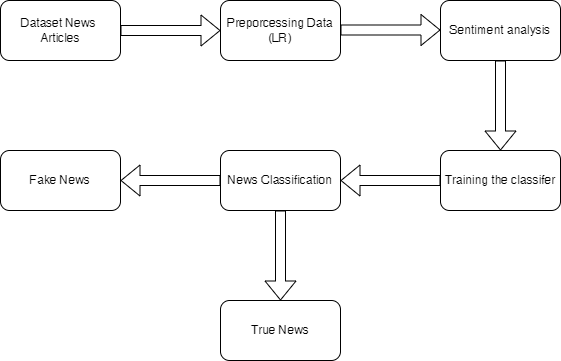
\includegraphics[height = 8cm]{Diagrams/New system.drawio.png}
    \caption{Main Architecture of System}
\end{figure}
\newpage
\subsection{Data Modelling(ER-Diagram)}
ER Diagram is mainly used to design database schema. With the help of below er diagram we can easily design database in SQL.
\begin{figure}[H]
    \rotatebox{90}{
    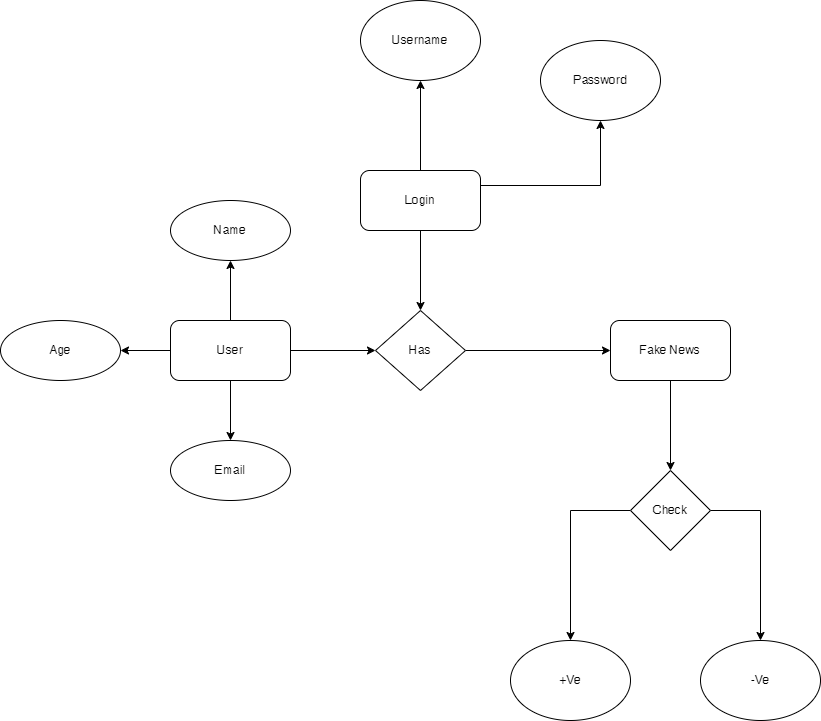
\includegraphics[height = 12cm]{Diagrams/ER new.drawio.png}}
    \caption{ER Diagram of System Data}
\end{figure}
\newpage
\subsection{Activity Diagram}
An activity diagram visually presents a series of actions or flow of control in a system similar to a flowchart or a data flow diagram. This diagram showed how our program flow goes on.
\begin{figure}[H]
   \centering
    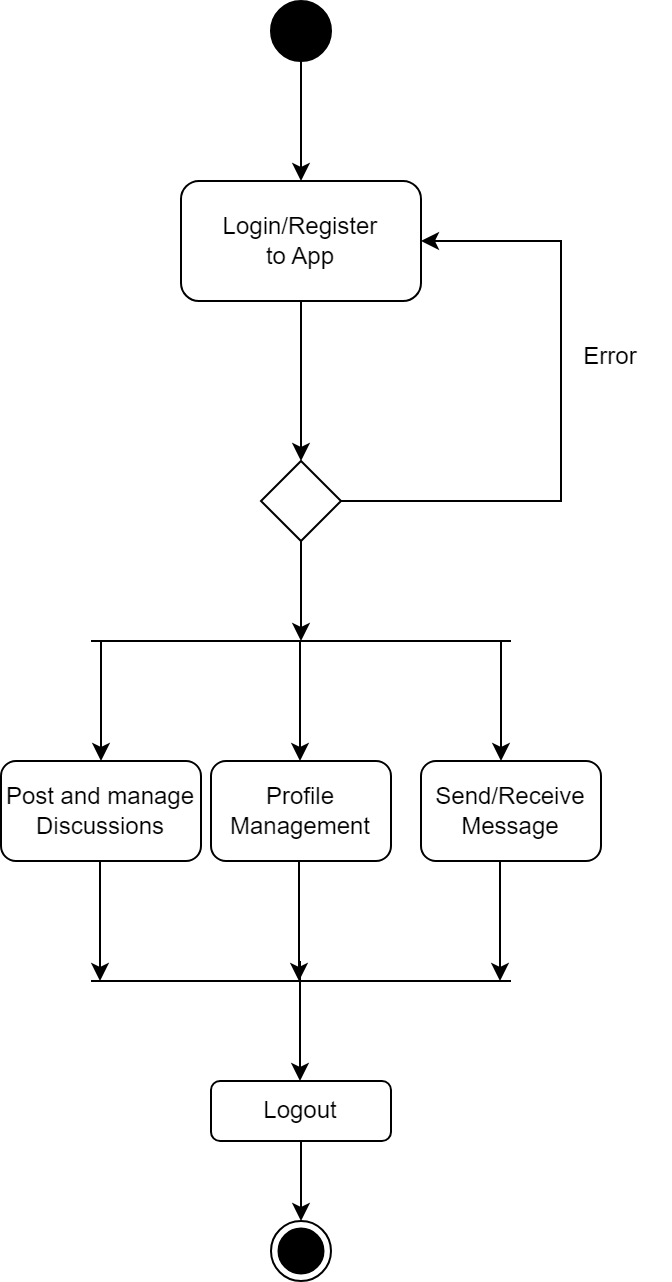
\includegraphics[height = 15cm]{Diagrams/Activity.drawio.png}
    \caption{Activity Diagram}
\end{figure}
\newpage
\subsection{DFD}
DFD or Data Flow Diagram is mainly used to show how data are being flowed in and out of our system. There are 3 levels of DFD i.e Context Level(Level 0),Level 1 and Level 2
\begin{figure}[H]
    \centering
    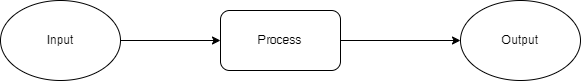
\includegraphics[height = 2cm]{Diagrams/dfd0new.drawio.png}
    \caption{Data Flow Diagram (Context Level)}
\end{figure}
\newpage
\subsection{Use Case Diagram}
A use case diagram, part of UML, visually represents interactions between actors and a system. Actors are external entities, while use cases depict specific functionalities. Relationships, such as association, generalization, include, and extend, illustrate connections between actors and use cases. The diagram helps in understanding system behavior, requirements, and scope.
\begin{figure}[H]
    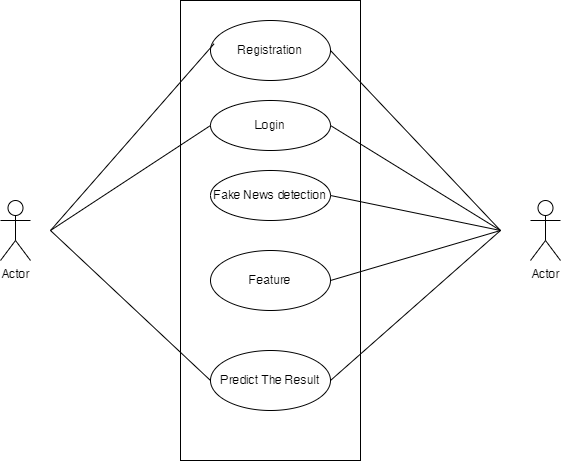
\includegraphics[height = 10cm]{Diagrams/Use-case.drawio.png}
    \caption{Use Case Diagram}
\end{figure}

\chapter{IMPLEMENTATION}


% (20\% of Report Length)

% a. Showcase the output at various intermediate stages of the project pipeline

% b. Use proper data visualizing techniques to present the output

% c. Figures and tables must be accompanied by an explanation
\section{Tools Used}
\textbf{Python}\\
Python is a versatile, high-level programming language known for its simplicity, readability, and extensive standard library. Developed in the late 1980s, Python's clear syntax supports multiple programming paradigms, including procedural and object-oriented styles. Its dynamic typing and interpreted nature facilitate rapid development and interactive debugging, making it popular across diverse domains such as web development, scientific computing, and artificial intelligence. Python's thriving community and robust ecosystem of libraries contribute to its widespread adoption and continued relevance in modern software development. \\
\textbf{Django}\\
Django is a high-level Python web framework designed for rapid development and clean, pragmatic design. Built on the principles of DRY (Don't Repeat Yourself) and convention over configuration, Django simplifies the creation of complex, database-driven websites by providing reusable components and a built-in admin interface. It encourages rapid development and clean, maintainable code through its "batteries-included" philosophy, offering features such as URL routing, template engine, ORM (Object-Relational Mapping), and authentication system out of the box. Django's scalability, security features, and extensive documentation make it a preferred choice for building robust web applications efficiently.
\\
\textbf{PostgreSQL}\\
PostgreSQL, often referred to as Postgres, is an advanced open-source relational database management system (RDBMS) known for its reliability, robustness, and extensibility. Developed over three decades with a strong emphasis on standards compliance and SQL features, PostgreSQL supports a wide range of data types, indexing techniques, and advanced features like full-text search and JSON support. It offers ACID (Atomicity, Consistency, Isolation, Durability) compliance, ensuring data integrity and reliability even in high-transaction environments. PostgreSQL's active community contributes to its continuous improvement and extensive documentation, making it a popular choice for applications requiring secure, scalable, and efficient data storage solutions.\\
\textbf{Git/Github}\\
Git is a distributed version control system (VCS) designed for managing software development projects and tracking changes to source code during development. Developed by Linus Torvalds in 2005, Git allows multiple developers to collaborate on projects simultaneously by maintaining a history of changes, facilitating code review, and enabling seamless integration of new features. Git operates locally on a developer's machine, providing branching and merging capabilities that support parallel development workflows and experimental features without affecting the main codebase. GitHub, on the other hand, is a web-based hosting service for Git repositories, offering additional features such as issue tracking, pull requests, and project management tools. It enhances collaboration and community engagement by providing a platform for developers to share, discuss, and contribute to open-source projects globally. Together, Git and GitHub form a powerful ecosystem that supports agile software development practices and fosters collaboration among developers worldwide.\\
\textbf{PyTorch}\\
PyTorch is an open-source machine learning library developed primarily by Facebook's AI Research lab (FAIR). It is widely used for building and training deep learning models, particularly neural networks, due to its dynamic computational graph and GPU acceleration capabilities. PyTorch emphasizes flexibility and ease of use, allowing developers to quickly prototype and experiment with different network architectures and algorithms. Key features include tensor computations with support for automatic differentiation, making it straightforward to implement and optimize complex neural networks. PyTorch is favored by researchers and practitioners in fields such as computer vision, natural language processing, and reinforcement learning for its intuitive API, extensive documentation, and active community support, making it a leading choice for cutting-edge machine learning projects. PyTorch is renowned for its seamless integration with Python.\\
\textbf{JavaScript}\\
JavaScript is a versatile programming language primarily used for creating dynamic and interactive web pages. Initially developed by Netscape in 1995, JavaScript has evolved into a fundamental tool for front-end web development, allowing developers to manipulate webpage content, handle events, and interact with users in real-time. It is widely supported by all modern web browsers and can be integrated with HTML and CSS to enhance user interfaces and create responsive web applications. JavaScript's asynchronous capabilities and extensive ecosystem of libraries and frameworks (such as React, Angular, and Vue.js) further contribute to its widespread use in both client-side and server-side development, making it essential for building modern, interactive web experiences.\\
% \textbf{React .js}\\
% React.js is a widely-used JavaScript library for creating efficient and reusable user interfaces. It offers a component-based architecture, virtual DOM for improved performance, and supports declarative programming. With a rich ecosystem of libraries and tools, React.js enables developers to build dynamic and responsive applications for both single-page and server-side rendering.\\
% \subsection{Implementation Details of Modules}
% \section{Testing}
% \subsection{Test Cases for Unit Testing}
% \subsection{Test Cases for System Testing}
\chapter{CONCLUSION AND EXPECTED OUTCOMES}
\section{Conclusion}
Code Connect is a social networking web application designed specifically for creative it professionals. It should transform the way developers connect, collaborate, and learn from each other. The platform provides a range of features that allow creative it professionals to network, share knowledge, and enhance their skills. Code Connect also fosters a vibrant and inclusive resume and portfolio management system.

\section{Expected Outcome}
Code Connect is a platform that aims to create a thriving community of creative it professionals who can connect, collaborate, and learn from each other. The platform provides tailored features that facilitate meaningful interactions and knowledge exchange among its users. Through Code Connect, creative it professionals can expect to expand their professional network, gain insights from experienced peers, and receive support from the community. They can engage in discussions, seek advice, and offer assistance. Code Connect also aims to accelerate the professional growth of its users by providing access to valuable resources, tutorials, and learning opportunities. By connecting with like-minded individuals and staying up-to-date with the latest trends and technologies, creative it professionals can enhance their skills and advance their careers. The platform's expected outcome is to create a vibrant and supportive ecosystem that empowers creative it professionals and enriches their professional lives.
In this complex world of technologies new peoples who are intrested in the field of technology face alot of difficulties.
So they will also have exposure with the help of out technology.

% ================================Appendices Setup================================================


\begin{appendices}
\renewcommand\thechapter{A}
\renewcommand\thefigure{\thechapter.\arabic{figure}}
\chapter*{APPENDIX A}
\addtocontents{toc}{\textbf{APPENDIX A}}
\section{Project Schedule}
Below is the Gantt chart of our project Schedule. We have planned to perfrom these specific tasks between these time frames.
\begin{figure}[H]
    \centering
        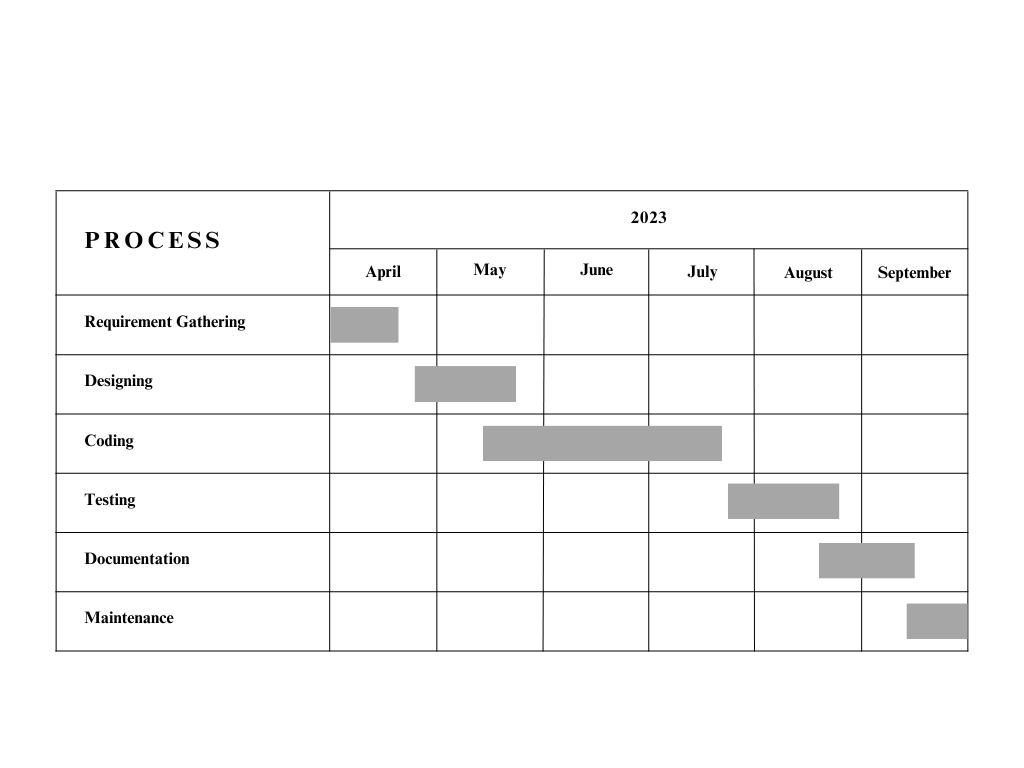
\includegraphics[width=400px]{Diagrams/Gantt_Chart.png}
    \caption{Gantt Chart of Schedule}
\end{figure}
\input{Appendix/appendix2.tex}
\end{appendices}



%========================References setup=========================================================
\newpage
\bibliographystyle{unsrt}
\bibliography{References/references}

\addcontentsline{toc}{chapter}{REFERENCES}

%=============================================================================================



%=========================================================================
\end{document}